\section{Data Needed}
In order to create a suitable database schema for the database that we want to create, we first need to figure out what will be in the database. This analysis focuses on the structure of the institutions involved in the GIRAF project. 

An institutions can have several departments. Each department has a number of employees, hereafter referred to as \emph{guardians}, assigned to it as well as some children that attend the department. Each department has one or more administrators, an administrator is a guardian with some extra privileges and authority. Each guardian is responsible for a few specific children, but is of course not limited to only taking care of to ones he is responsible for - the same applies to administrators. This is however something that they handle internally and it is more of a formality i.e. The schema of which children each guardian takes care of is quite flexible and generally all of the guardians take care of all of the children at their departments. As \autoref{fig:data_overview} illustrates, each department has a number of guardians and children and one of the guardians acts as an administrator for that department. Children are assigned to one specific department. Generally each department has it's own administrators, but in some cases a single administrator handles several departments.

\begin{figure}[hptb]
	\begin{center}
	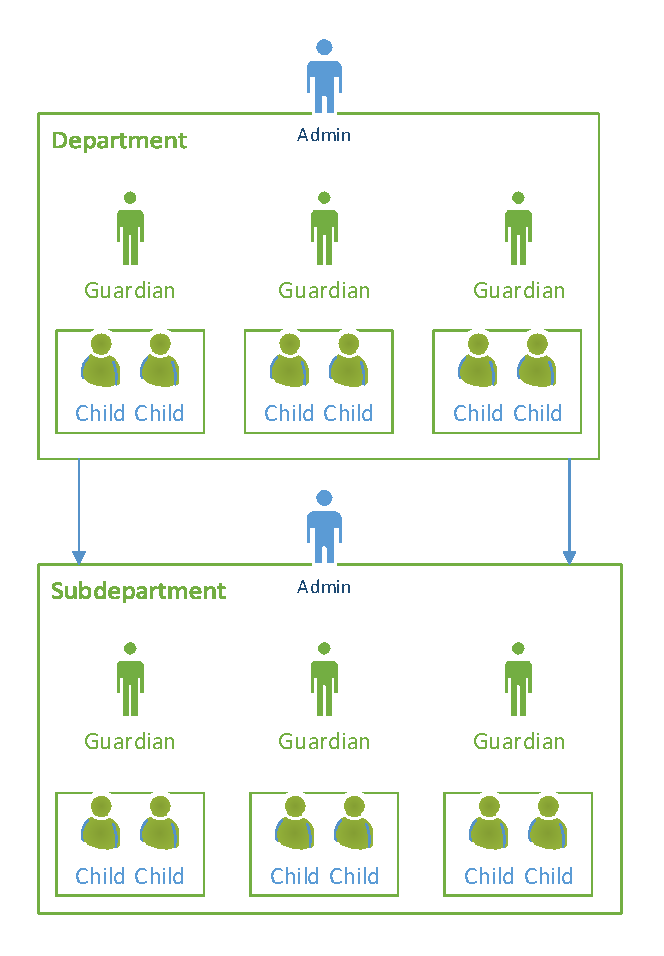
\includegraphics[width=0.8\textwidth]{img/data_overview.pdf}
	\label{fig:data_overview}
	\caption{Overview of the people involved and department structure}
	\end{center}
\end{figure} 

The children have some needs and demands that can vary greatly from one child to another. But common for all of the children is that they each have their own set of pictograms. The children generally have a resistance to change e.g. the taxi that drives them to the institution and picks them up again has to have a specific color. This tendency can also occur with regard to preferences as some children insist on their pictograms being black on white with stick figure and other prefer colored images. 

When these things are applied to what could be used in the database schema, we need to be able to represent \emph{departments} with optional \emph{subdepartments}. There needs to be a to representation of \emph{guardians} and \emph{children}. We also need to be able to give guardians \emph{administrator} rights to departments. The \emph{pictograms} also need to be included and it might be a good idea to be able to categorize the pictograms e.g. cereal and milk under breakfast items.

%\begin{figure}
%	\begin{center}
%	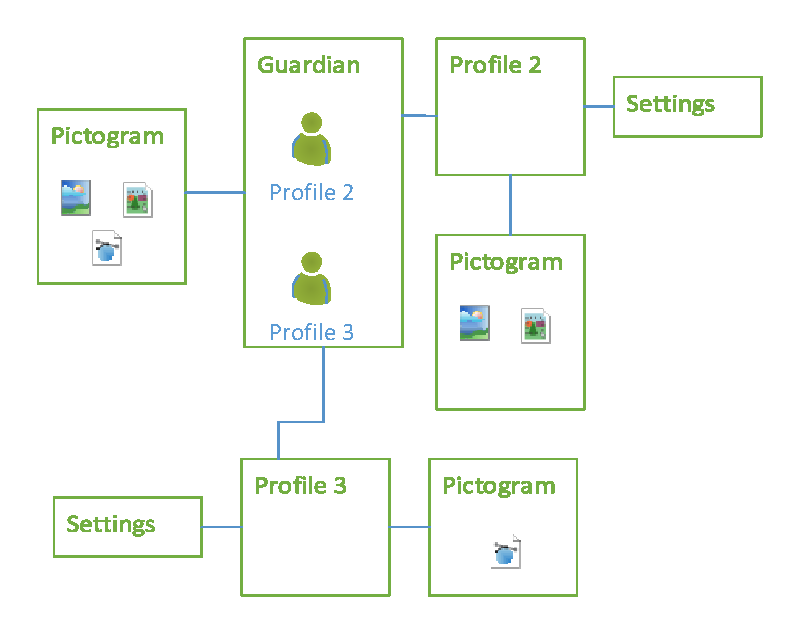
\includegraphics[width=\textwidth]{img/child_guardian.pdf}
%	\end{center}
%	\label{fig:child_guardian}
%	\caption{Illustration of the relationship between guardian and children}
%\end{figure} 

%One approach could be, to have a profile entity that can cover over both children and guardians. A specific profile could then be guardian of a number of other profiles. If a profile is not guardian of other profiles then it is a child profile. The profile can have his own preferences in games and have a custom set of pictograms. And will of course be assigned to a department. \autoref{fig:child_guardian} illustrates this relationship where the guardian has access to the children's profiles. All of the profiles have their own set of pictograms assigned to them and the guardian has the authority to edit in it's children's pictograms.


